\chapter{计算复杂性理论}

\section{时间/空间复杂度}

\subsection{算法(Algorithm)}

算法是解决问题的一种方法,由一系列的步骤组成。算法有5个特点:

\begin{enumerate}
	\item 有穷性(finiteness):算法必须在有限个步骤后终止。
	\item 确定性(definiteness):算法的每个步骤必须有确切的定义。
	\item 输入项(input):一个算法有0个或多个输入。
	\item 输出项(output):一个算法有1个或多个输出,没有输出的算法是毫无意义的。
	\item 可行性(effectiveness):算法中执行的任何步骤都可以被分解为基本的可执行操作。
\end{enumerate}

\vspace{0.5cm}

\subsection{时间复杂度(Time Complexity)}

算法有高效的,也有拙劣的。衡量算法好坏的标准有时间复杂度和空间复杂度。\\

想象一个场景:老板让小灰和大黄完成一个需求,两人都完成并交付了各自的代码,代码的功能是一样的。但是,大黄的代码运行一次要花100ms,占用5MB内存;小灰的代码运行一次要花100s,占用500MB内存。\\

“小灰,收拾东西走人,明天不用来上班了!”\\

小灰虽然也按照老板的要求实现了功能,但他的代码存在很严重的问题:运行时间长、占用空间大。\\

算法的时间复杂度是指算法中基本运算的执行次数,其中基本运算指的是加减法、交换、比较等操作。\\

算法的效率应该取决于算法本身,与机器无关。分析算法运行效率时应该考虑的是运行时间与输入规模之间的关系。通过计算算法中基本运算的执行次数,可以得到一个关于输入规模$ n $的函数。\\

时间复杂度一般采用大O表示法,表示算法的运行时间与输入规模之间的增长关系。常见的时间复杂度包括$ O(1) $、$ O(logn) $、$ O(n) $、$ O(nlogn) $、$ O(n^2) $、$ O(2^n) $、$ O(n!) $等。\\

时间复杂度需要满足以下原则:

\begin{enumerate}
	\item 如果运行时间是常量级,则用$ O(1) $表示。
	\item 只保留时间函数中的最高阶项。
	\item 如果最高阶项存在,则省去最高阶项前的系数。
\end{enumerate}

\vspace{0.5cm}

\subsubsection{大O符号}

大O符号用于表示时间复杂度的上界(最坏情况),即算法的阶不会超过大O符号中的函数$ f(n) $。

\vspace{-0.5cm}

\begin{align}
	0 \le f(n) \le cg(n)
\end{align}

\vspace{-1cm}

\begin{align*}
	f(n) & = n^2 + n \\
	     & = O(n^2)  \\
	     & = O(n^3)
\end{align*}

\subsubsection{大$ \Omega $符号}

大$ \Omega $符号用于表示时间复杂度的下界(最好情况),即算法的阶不会低于大$ \Omega $符号中的函数$ f(n) $。

\vspace{-0.5cm}

\begin{align}
	0 \le cg(n) \le f(n)
\end{align}

\vspace{-1cm}

\begin{align*}
	f(n) & = n^2 + n      \\
	     & = \Omega(n^2)  \\
	     & = \Omega(100n)
\end{align*}

\subsubsection{小o符号}

小o符号用于表示时间复杂度的上界,即算法的阶一定低于小o符号中的函数$ f(n) $。

\vspace{-0.5cm}

\begin{align}
	0 \le f(n) < cg(n)
\end{align}

\vspace{-1cm}

\begin{align*}
	f(n) & = n^2 + n \\
	     & = o(n^3)
\end{align*}

\subsubsection{小$ \omega $符号}

小$ \omega $符号用于表示时间复杂度的下界,即算法的阶一定高于小$ \omega $符号中的函数$ f(n) $。

\vspace{-0.5cm}

\begin{align}
	0 \le cg(n) < f(n)
\end{align}

\vspace{-1cm}

\begin{align*}
	f(n) & = n^2 + n     \\
	     & = \omega(n^2)
\end{align*}

\subsubsection{$ \Theta $符号}

若$ f(n) = O(g(n)) $且$ f(n) = \Omega(g(n)) $,则称$ f(n) $的阶与$ g(n) $的阶相等:

\vspace{-0.5cm}

\begin{align}
	f(n) = \Theta(g(n))
\end{align}

\vspace{-1cm}

\begin{align*}
	f(n) & = n^2 + n     \\
	g(n) & = 100n^2      \\
	     & = \Theta(n^2)
\end{align*}

\vspace{0.5cm}

\mybox{百钱买百鸡}\\

公鸡5文钱1只,母鸡3文钱1只,小鸡1文钱3只,如果用100文钱买100只鸡,那么公鸡、母鸡和小鸡各应该买多少只?

\begin{lstlisting}[language=C]
void buy(int n, int money) {
	for (int x = 0; x <= n / 5; x++) {
		for (int y = 0; y <= n / 3; y++) {
			int z = n - x - y;
			if (z > 0 && z % 3 == 0 && 5*x + 3*y + z/3 == money) {
				printf("x = %d, y = %d, z = %d\n", x, y, z);
			}
		}
	}
}
\end{lstlisting}

\vspace{0.5cm}

\subsection{空间复杂度(Space Complexity)}

算法占用的内存空间自然是越小越好,空间复杂度是对一个算法在运行过程中临时占用存储空间大小的量度,它同样使用了大O表示法。\\

正所谓鱼和熊掌不可兼得,很多时候不得不在时间复杂度和空间复杂度之间进行取舍。绝大多数时候,时间复杂度更为重要,宁可多分配一些内存空间,也要提升程序的执行速度。

\vspace{0.5cm}

\subsection{均摊时间复杂度(Amortized Time Complexity)}

均摊时间复杂度用于分析一组操作中,虽然某个操作的时间复杂度很高,但是经过若干次操作后,这组操作的平均时间复杂度较低的情况。\\

\mybox{动态数组}

\begin{lstlisting}[language=Java]
public void add(T element) {
	if (size == capacity) {
		capacity *= 2;
		T[] newArr = (T[]) new Object[capacity];
		System.arraycopy(arr, 0, newArr, 0, size);
		arr = newArr;
	}
	arr[size++] = element;
}
\end{lstlisting}

这段代码实现了往数组中添加数据的功能。在数组没有满的情况下,直接将数据添加到数组末尾,时间复杂度为$ O(1) $。\\

但是当数组已满时,需要对数组创建一个更大的数组,将原数组中的数据复制到新数组中,然后再将新数据添加到数组的末尾,这个过程的时间复杂度为$ O(n) $。\\

假设数组的容量为$ n $,每执行$ n $次add()操作,才会进行一次扩容。那么,可以将这一次的$ O(n) $的时间均摊到前面的$ n $次操作中,这样add()操作的均摊时间复杂度就是$ O(1) $。

\newpage

\section{递推方程}

\subsection{递推(Recurrence)}

递归算法无法直接根据语句的执行次数计算出时间复杂度,但是可以通过递推方程迭代展开进行求解。\\

\mybox{求和}

\begin{lstlisting}[language=C]
int sum(int n) {
	if (n <= 0) {
		return 0;
	}
	return sum(n - 1) + n;
}
\end{lstlisting}

\vspace{-0.5cm}

\begin{align}
	T(n) = \begin{cases}
		1          & n = 0   \\
		T(n-1) + 1 & n \ge 1
	\end{cases}
\end{align}

\vspace{-1cm}

\begin{align*}
	T(n) & = T(n-1) + 1                \\
	     & = [T(n-2) + 1] + 1          \\
	     & = [[T(n-3) + 1] + 1] + 1    \\
	     & = \dots                     \\
	     & = T(n-k) + k                \\
	\\
	     & n - k = 0 \Rightarrow n = k \\
	\\
	T(n) & = T(n-n) + n                \\
	     & = T(0) + n                  \\
	     & = 1 + n                     \\
	     & = O(n)
\end{align*}

\vspace{0.5cm}

\mybox{插入排序}

\begin{lstlisting}[language=C]
void insert_sort(int arr[], int n) {
    if (n <= 1) {
		return;
	}
    insert_sort(arr, n-1);
    int last = arr[n-1];
    int j = n - 2;
    while (j >= 0 && arr[j] > last) {
        arr[j+1] = arr[j];
        j--;
    }
    arr[j+1] = last;
}
\end{lstlisting}

\vspace{-0.5cm}

\begin{align}
	T(n) = \begin{cases}
		1          & n <= 1  \\
		T(n-1) + n & n \ge 1
	\end{cases}
\end{align}

\vspace{-1cm}

\begin{align*}
	T(n) & = T(n-1) + n                \\
	     & = [T(n-2) + n] + n          \\
	     & = [[T(n-3) + n] + n] + n    \\
	     & = \dots                     \\
	     & = T(n-k) + nk               \\
	\\
	     & n - k = 0 \Rightarrow n = k \\
	\\
	T(n) & = T(n-n) + n^2              \\
	     & = T(0) + n^2                \\
	     & = 1 + n^2                   \\
	     & = O(n^2)
\end{align*}

\vspace{0.5cm}

\mybox{汉诺塔}\\

有三根柱子A、B、C,A柱子上从下到上套有n个圆盘,要求将A柱子上的圆盘移动到C柱子上。每次只能移动一个圆盘,且大圆盘始终不能叠在小圆盘上面。\\

\begin{figure}[H]
	\centering
	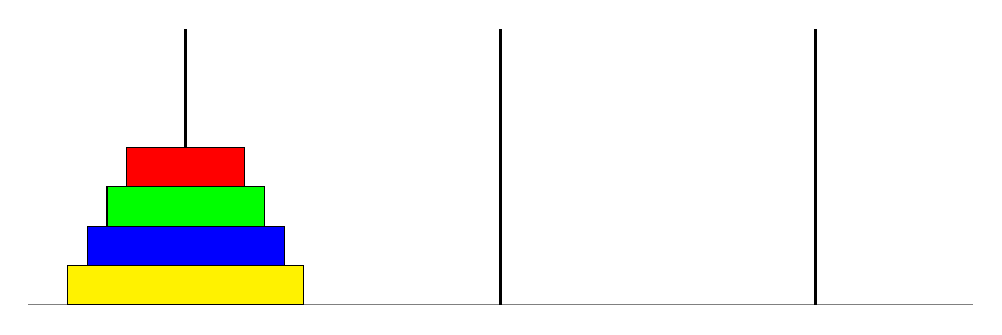
\begin{tikzpicture}[scale=0.5]
		\draw[-, gray] (0,0) -- (24,0);
		\draw[-, very thick] (4,0) -- (4,7);
		\draw[-, very thick] (12,0) -- (12,7);
		\draw[-, very thick] (20,0) -- (20,7);

		\draw[fill=red] (2.5,3) rectangle (5.5,4);
		\draw[fill=green] (2,2) rectangle (6,3);
		\draw[fill=blue] (1.5,1) rectangle (6.5,2);
		\draw[fill=yellow] (1,0) rectangle (7,1);
	\end{tikzpicture}
	\caption{汉诺塔}
\end{figure}

递归算法求解汉诺塔问题:

\begin{enumerate}
	\item 将前n - 1个圆盘从A柱借助于C柱搬到B柱。
	\item 将最后一个圆盘直接从A柱搬到C柱。
	\item 将n - 1个圆盘从B柱借助于A柱搬到C柱。
\end{enumerate}

\vspace{-0.5cm}

\begin{lstlisting}[language=Python]
def hanoi(n, A, B, C):
    if n == 1
        move(1, A, C)
    else
        hanoi(n-1, A, C, B)
        move(n, A, C)
        hanoi(n-1, B, A, C)
\end{lstlisting}

\vspace{-0.5cm}

\begin{align}
	T(n) = \begin{cases}
		1           & n = 1 \\
		2T(n-1) + 1 & n > 1
	\end{cases}
\end{align}

\vspace{-1cm}

\begin{align*}
	T(n) & = 2T(n-1) + 1                   \\
	     & = 2[2T(n-2) + 1] + 1            \\
	     & = 2[2[2T(n-3) + 1] + 1] + 1     \\
	     & = \dots                         \\
	     & = 2^k * T(n-k) + 2^k - 1        \\
	\\
	     & n - k = 1 \Rightarrow n = k + 1 \\
	\\
	T(n) & = 2^{n-1} * T(1) + 2^{n-1} - 1  \\
	     & = 2^{n-1} + 2^{n-1} - 1         \\
	     & = 2^n - 1                       \\
	     & = O(2^n)
\end{align*}

假设每次移动花费1秒,解决一个64层的汉诺塔问题大约需要5800亿年。\\

\begin{figure}[H]
	\centering
	\includegraphics[]{img/Chapter1/1-2/1.png}
\end{figure}

\newpage

\section{P=NP?}

\subsection{旅行商问题(Traveling Salesman Problem)}

小灰最近在工作中遇到了一个棘手的问题。公司正在开发一个物流项目,其中一个需求是为快递员自动规划送快递的路线。\\

有一个快递员,要分别给三家顾客送快递,他自己到达每个顾客家的路程各不相同,每个顾客之间的路程也各不相同。那么想要把快递依次送达这三家,并最终回到起点,哪一条路线所走的总距离是最短的呢?

\begin{figure}[H]
	\centering
	\begin{tikzpicture}
		\begin{scope}[every node/.style={circle,thick,draw}]
			\node (A) at (0,0) {出发};
			\node (B) at (-4,3) {客户};
			\node (C) at (1,7) {客户};
			\node (D) at (3,3) {客户};
		\end{scope}

		\begin{scope}[>={Stealth[black]},
			every node/.style={fill=white,circle},
			every edge/.style={draw=black,very thick}]
			\path [-] (A) edge node {2} (B);
			\path [-] (A) edge node {5} (C);
			\path [-] (A) edge node {6} (D);
			\path [-] (B) edge node {3} (C);
			\path [-] (B) edge node {4} (D);
			\path [-] (C) edge node {7} (D);
		\end{scope}
	\end{tikzpicture}
	\caption{快递客户路线}
\end{figure}

为了寻求最优路线,小灰研究了好久,可惜还是没有找到一个高效率的解决方案。不只是小灰,当前的计算机科学家们也没有找到一个行之有效的优化方案,这是典型的旅行商问题。\\

有一个商品推销员,要去若干个城市推销商品。该推销员从一个城市出发,需要经过所有城市后,回到出发地。每个城市之间都有道路连通,且距离各不相同,推销员应该如何选择路线,使得总行程最短呢?\\

这个问题看起来很简单,却很难找到一个真正高效的求解算法。其中最容易想到的,是使用穷举法把所有可能的路线穷举出来,计算出每一条路线的总行程。通过排列组合,从所有路线中找出总行程最短的路线。显然,这个方法的时间复杂度是$ O(n!) $,随着城市数量的增长,花费的运算时间简直不可想象!\\

后来,人们想出了许多相对优化的解决方案,比如动态规划法和分枝定界法等。但是,这些算法的时间复杂度仍然是指数级的,并没有让性能问题得到根本的解决。\\

像这样的问题有很多,旅行商问题仅仅是其中的一例。对于这类问题统称为NP问题。\\

\subsection{P=NP?}

算法的设计与分析在计算机科学领域有着重要的应用背景。1966 $ \sim $ 2005年期间,Turing奖获奖50人,其中10人以算法设计,7人以计算理论、自动机和复杂性研究领域的杰出贡献获奖。计算复杂性理论中的P=NP?问题是世界七大数学难题之一。\\

一些常见的算法的时间复杂度,例如二分查找法$ O(logn) $、归并排序$ O(nlogn) $、Floyd最短路径$ O(n^3) $等,都可以用$ O(n^k) $表示。这些算法都是多项式时间算法,即能在多项式时间内解决问题。这类问题被称为P问题(Polynomial)。\\

人们常说,能用钱解决的问题都不是问题。在计算机科学家眼中,能用多项式时间解决的问题都不是问题。\\

然而,世间还存在许多变态的问题,是无法(至少是暂时无法)在多项式时间内解决的,比如一些算法的时间复杂度是$ O(2^n) $,甚至$ O(n!) $。随着问题规模$ n $的增长,计算量的增长速度是非常恐怖的。这类问题被称为NP问题(Non-deterministic Polynomial),意思是“不确定是否能在多项式时间内解决”。\\

有些科学家认为,所有的NP问题终究都可以在多项式时间内解决,只是我们暂时还没有找到方法;也有些科学家认为,某些NP问题永远无法在多项式时间内解决。这个业界争论用P=NP?这个公式来表达。\\

这还不算完,在所有的NP问题当中,还存在着一些大BOSS,被称为NPC问题。\\

\subsection{NPC}

这里所说的NPC问题可不是游戏当中的NPC。要想理解NPC问题,需要先了解归约的概念。\\

归约(reduction)可以简单理解成问题之间的转化。例如问题是一个一元一次方程的求解问题$ Q: 3x + 6 = 12 $,这个问题可以转化成一个一元二次方程$ Q': 0x^2 + 3x + 6 = 12 $。\\

问题$ Q $并不比问题$ Q' $难解决,只要有办法解决$ Q' $,就一定能够解决$ Q $。对于这种情况,可以说问题$ Q $归约于问题$ Q' $。\\

同时,这种归约可以逐级传递,比如问题A归约于问题B,问题B归约于问题C,问题C归约于问题D,那么可以说问题A归约于问题D。\\

在NP问题之间,也可以存在归约关系。把众多的NP问题层层归约,必定会得到一个或多个终极问题,这些归约的终点就是所谓的NPC问题(NP-Complete)。旅行商问题被科学家证明属于NPC问题。\\

俗话说擒贼先擒王,只要有朝一日,我们能够找到NPC问题的多项式时间算法,就能够解决掉所有的NP问题!但遗憾的是,至今还没有人能够找到可行的方法,很多人认为这个问题是无解的。\\

回到最初的快递路线规划问题,既然是工程问题,与其钻牛角尖寻求最优解,不如用小得多的代价寻求次优解。最简单的办法是使用贪心算法,先选择距离起点最近的地点A,再选择距离A最近的地点B,以此类推,每一步都保证局部最优。这样规划出的路线未必是全局最优,但平均情况下也不会比最优方案差多少。

\newpage